\documentclass[]{article}
\usepackage{lmodern}
\usepackage{amssymb,amsmath}
\usepackage{ifxetex,ifluatex}
\usepackage{fixltx2e} % provides \textsubscript
\ifnum 0\ifxetex 1\fi\ifluatex 1\fi=0 % if pdftex
  \usepackage[T1]{fontenc}
  \usepackage[utf8]{inputenc}
\else % if luatex or xelatex
  \ifxetex
    \usepackage{mathspec}
    \usepackage{xltxtra,xunicode}
  \else
    \usepackage{fontspec}
  \fi
  \defaultfontfeatures{Mapping=tex-text,Scale=MatchLowercase}
  \newcommand{\euro}{€}
\fi
% use upquote if available, for straight quotes in verbatim environments
\IfFileExists{upquote.sty}{\usepackage{upquote}}{}
% use microtype if available
\IfFileExists{microtype.sty}{%
\usepackage{microtype}
\UseMicrotypeSet[protrusion]{basicmath} % disable protrusion for tt fonts
}{}
\usepackage[margin=1in]{geometry}
\ifxetex
  \usepackage[setpagesize=false, % page size defined by xetex
              unicode=false, % unicode breaks when used with xetex
              xetex]{hyperref}
\else
  \usepackage[unicode=true]{hyperref}
\fi
\hypersetup{breaklinks=true,
            bookmarks=true,
            pdfauthor={},
            pdftitle={Residuals},
            colorlinks=true,
            citecolor=blue,
            urlcolor=blue,
            linkcolor=magenta,
            pdfborder={0 0 0}}
\urlstyle{same}  % don't use monospace font for urls
\usepackage{color}
\usepackage{fancyvrb}
\newcommand{\VerbBar}{|}
\newcommand{\VERB}{\Verb[commandchars=\\\{\}]}
\DefineVerbatimEnvironment{Highlighting}{Verbatim}{commandchars=\\\{\}}
% Add ',fontsize=\small' for more characters per line
\usepackage{framed}
\definecolor{shadecolor}{RGB}{248,248,248}
\newenvironment{Shaded}{\begin{snugshade}}{\end{snugshade}}
\newcommand{\KeywordTok}[1]{\textcolor[rgb]{0.13,0.29,0.53}{\textbf{{#1}}}}
\newcommand{\DataTypeTok}[1]{\textcolor[rgb]{0.13,0.29,0.53}{{#1}}}
\newcommand{\DecValTok}[1]{\textcolor[rgb]{0.00,0.00,0.81}{{#1}}}
\newcommand{\BaseNTok}[1]{\textcolor[rgb]{0.00,0.00,0.81}{{#1}}}
\newcommand{\FloatTok}[1]{\textcolor[rgb]{0.00,0.00,0.81}{{#1}}}
\newcommand{\ConstantTok}[1]{\textcolor[rgb]{0.00,0.00,0.00}{{#1}}}
\newcommand{\CharTok}[1]{\textcolor[rgb]{0.31,0.60,0.02}{{#1}}}
\newcommand{\SpecialCharTok}[1]{\textcolor[rgb]{0.00,0.00,0.00}{{#1}}}
\newcommand{\StringTok}[1]{\textcolor[rgb]{0.31,0.60,0.02}{{#1}}}
\newcommand{\VerbatimStringTok}[1]{\textcolor[rgb]{0.31,0.60,0.02}{{#1}}}
\newcommand{\SpecialStringTok}[1]{\textcolor[rgb]{0.31,0.60,0.02}{{#1}}}
\newcommand{\ImportTok}[1]{{#1}}
\newcommand{\CommentTok}[1]{\textcolor[rgb]{0.56,0.35,0.01}{\textit{{#1}}}}
\newcommand{\DocumentationTok}[1]{\textcolor[rgb]{0.56,0.35,0.01}{\textbf{\textit{{#1}}}}}
\newcommand{\AnnotationTok}[1]{\textcolor[rgb]{0.56,0.35,0.01}{\textbf{\textit{{#1}}}}}
\newcommand{\CommentVarTok}[1]{\textcolor[rgb]{0.56,0.35,0.01}{\textbf{\textit{{#1}}}}}
\newcommand{\OtherTok}[1]{\textcolor[rgb]{0.56,0.35,0.01}{{#1}}}
\newcommand{\FunctionTok}[1]{\textcolor[rgb]{0.00,0.00,0.00}{{#1}}}
\newcommand{\VariableTok}[1]{\textcolor[rgb]{0.00,0.00,0.00}{{#1}}}
\newcommand{\ControlFlowTok}[1]{\textcolor[rgb]{0.13,0.29,0.53}{\textbf{{#1}}}}
\newcommand{\OperatorTok}[1]{\textcolor[rgb]{0.81,0.36,0.00}{\textbf{{#1}}}}
\newcommand{\BuiltInTok}[1]{{#1}}
\newcommand{\ExtensionTok}[1]{{#1}}
\newcommand{\PreprocessorTok}[1]{\textcolor[rgb]{0.56,0.35,0.01}{\textit{{#1}}}}
\newcommand{\AttributeTok}[1]{\textcolor[rgb]{0.77,0.63,0.00}{{#1}}}
\newcommand{\RegionMarkerTok}[1]{{#1}}
\newcommand{\InformationTok}[1]{\textcolor[rgb]{0.56,0.35,0.01}{\textbf{\textit{{#1}}}}}
\newcommand{\WarningTok}[1]{\textcolor[rgb]{0.56,0.35,0.01}{\textbf{\textit{{#1}}}}}
\newcommand{\AlertTok}[1]{\textcolor[rgb]{0.94,0.16,0.16}{{#1}}}
\newcommand{\ErrorTok}[1]{\textcolor[rgb]{0.64,0.00,0.00}{\textbf{{#1}}}}
\newcommand{\NormalTok}[1]{{#1}}
\usepackage{graphicx,grffile}
\makeatletter
\def\maxwidth{\ifdim\Gin@nat@width>\linewidth\linewidth\else\Gin@nat@width\fi}
\def\maxheight{\ifdim\Gin@nat@height>\textheight\textheight\else\Gin@nat@height\fi}
\makeatother
% Scale images if necessary, so that they will not overflow the page
% margins by default, and it is still possible to overwrite the defaults
% using explicit options in \includegraphics[width, height, ...]{}
\setkeys{Gin}{width=\maxwidth,height=\maxheight,keepaspectratio}
\setlength{\parindent}{0pt}
\setlength{\parskip}{6pt plus 2pt minus 1pt}
\setlength{\emergencystretch}{3em}  % prevent overfull lines
\providecommand{\tightlist}{%
  \setlength{\itemsep}{0pt}\setlength{\parskip}{0pt}}
\setcounter{secnumdepth}{0}

%%% Use protect on footnotes to avoid problems with footnotes in titles
\let\rmarkdownfootnote\footnote%
\def\footnote{\protect\rmarkdownfootnote}

%%% Change title format to be more compact
\usepackage{titling}

% Create subtitle command for use in maketitle
\newcommand{\subtitle}[1]{
  \posttitle{
    \begin{center}\large#1\end{center}
    }
}

\setlength{\droptitle}{-2em}

  \title{Residuals}
    \pretitle{\vspace{\droptitle}\centering\huge}
  \posttitle{\par}
    \author{}
    \preauthor{}\postauthor{}
    \date{}
    \predate{}\postdate{}
  
% Redefines (sub)paragraphs to behave more like sections
\ifx\paragraph\undefined\else
\let\oldparagraph\paragraph
\renewcommand{\paragraph}[1]{\oldparagraph{#1}\mbox{}}
\fi
\ifx\subparagraph\undefined\else
\let\oldsubparagraph\subparagraph
\renewcommand{\subparagraph}[1]{\oldsubparagraph{#1}\mbox{}}
\fi


\begin{document}
\maketitle

Let's begin by considering some specific residuals from our data.
Suppose we are interested in making a prediction about the student in
row 12, a vegetarian whose favorite celebrity is Michelle Obama. Let's
study that row of data:

\begin{Shaded}
\begin{Highlighting}[]
\KeywordTok{require}\NormalTok{(mosaic)}
\CommentTok{# install.packages("googlesheets")}
\KeywordTok{require}\NormalTok{(googlesheets)}
\NormalTok{url =}\StringTok{ }\KeywordTok{gs_url}\NormalTok{(}\StringTok{"https://docs.google.com/spreadsheets/d/1tHg_Oo88GIS8E00-lf286-4AzR-wht7ZddUMFM1s5s0/"}\NormalTok{)}
\NormalTok{ds =}\StringTok{ }\KeywordTok{gs_read_csv}\NormalTok{(url)}

\NormalTok{ds %>%}\StringTok{ }\KeywordTok{slice}\NormalTok{(}\DecValTok{12}\NormalTok{)}
\end{Highlighting}
\end{Shaded}

This student has 623 facebook friends and has had an account for 7
years. We could also look at row 10,

\begin{Shaded}
\begin{Highlighting}[]
\NormalTok{ds %>%}\StringTok{ }\KeywordTok{slice}\NormalTok{(}\DecValTok{10}\NormalTok{)}
\end{Highlighting}
\end{Shaded}

This student has 320 friends and an account for 5 years. But, what are
the predicted values for those students?

\begin{Shaded}
\begin{Highlighting}[]
\NormalTok{mod =}\StringTok{ }\KeywordTok{lm}\NormalTok{(numFBFriends ~}\StringTok{ }\NormalTok{accountLength, }\DataTypeTok{data=}\NormalTok{ds)}
\KeywordTok{summary}\NormalTok{(mod)}
\KeywordTok{xyplot}\NormalTok{(numFBFriends ~}\StringTok{ }\NormalTok{accountLength, }\DataTypeTok{data=}\NormalTok{ds, }\DataTypeTok{type=}\KeywordTok{c}\NormalTok{(}\StringTok{"p"}\NormalTok{, }\StringTok{"r"}\NormalTok{))}
\NormalTok{new_ds =}\StringTok{ }\KeywordTok{data.frame}\NormalTok{(}\DataTypeTok{accountLength =} \KeywordTok{c}\NormalTok{(}\DecValTok{7}\NormalTok{, }\DecValTok{5}\NormalTok{))}
\KeywordTok{predict}\NormalTok{(mod, }\DataTypeTok{newdata =} \NormalTok{new_ds)}
\end{Highlighting}
\end{Shaded}

So, it predicts that the first student would have 1006 friends, and the
second student would have 837 friends. What are their residuals?

\begin{Shaded}
\begin{Highlighting}[]
\DecValTok{623} \NormalTok{-}\StringTok{ }\DecValTok{584}
\DecValTok{320} \NormalTok{-}\StringTok{ }\DecValTok{415}
\end{Highlighting}
\end{Shaded}

One is positive, one is negative. We can also look at the residuals for
the entire class, or compute the Sum of Squared Residuals (SSR).

\begin{Shaded}
\begin{Highlighting}[]
\KeywordTok{residuals}\NormalTok{(mod)}
\KeywordTok{sum}\NormalTok{(}\KeywordTok{residuals}\NormalTok{(mod)^}\DecValTok{2}\NormalTok{) }
\end{Highlighting}
\end{Shaded}

Finally, we could take the mean of the residuals

\begin{Shaded}
\begin{Highlighting}[]
\KeywordTok{mean}\NormalTok{(}\KeywordTok{residuals}\NormalTok{(mod))}
\end{Highlighting}
\end{Shaded}

(the sum is essentially 0)

\subsection{Assessing conditions for
regression}\label{assessing-conditions-for-regression}

Let's try to assess the conditions for regression on this example. The
easiest way to do this is to run the \texttt{plot()} command on your
model object,

\begin{Shaded}
\begin{Highlighting}[]
\KeywordTok{plot}\NormalTok{(mod, }\DataTypeTok{which=}\KeywordTok{c}\NormalTok{(}\DecValTok{1}\NormalTok{,}\DecValTok{2}\NormalTok{))}
\end{Highlighting}
\end{Shaded}

We'll focus on the first two plots for now (if you don't specify
\texttt{which}, you will get four plots). The first is the residual
versus fitted values plot, which helps us assess linearity and equality
of variance, and the second is a QQ plot (quantile-quantile plot) to
help us assess normality. Another way to assess normality of the
residuals is to make a histogram.

\begin{Shaded}
\begin{Highlighting}[]
\KeywordTok{histogram}\NormalTok{(~residuals, }\DataTypeTok{data=}\NormalTok{mod, }\DataTypeTok{fit=}\StringTok{"normal"}\NormalTok{)}
\end{Highlighting}
\end{Shaded}

\subsection{Pathological examples}\label{pathological-examples}

Because most real models are hard to assess, we want to examine some
pathological examples of the LINE conditions for regression being
violated.

For all these examples, we will generate simulated data to show the
particular conditions being violated.

You'll notice that even as we're trying to simulate data to violate one
condition, the others start to look bad, too. This is very common in the
real world, as well!

\paragraph{Good Model}\label{good-model}

First, a positive example! Let's make some good data.

\begin{Shaded}
\begin{Highlighting}[]
\KeywordTok{require}\NormalTok{(mosaic)}
\NormalTok{n =}\StringTok{ }\DecValTok{10000}
\NormalTok{beta0 =}\StringTok{ }\DecValTok{10}
\NormalTok{beta1 =}\StringTok{ }\DecValTok{3}
\NormalTok{x =}\StringTok{ }\KeywordTok{runif}\NormalTok{(n)}
\NormalTok{e =}\StringTok{ }\KeywordTok{rnorm}\NormalTok{(n)}
\NormalTok{ds =}\StringTok{ }\KeywordTok{data.frame}\NormalTok{(}\DataTypeTok{y =} \NormalTok{beta0 +}\StringTok{ }\NormalTok{beta1 *}\StringTok{ }\NormalTok{x +}\StringTok{ }\NormalTok{e)}
\end{Highlighting}
\end{Shaded}

Now, we can look at the relationship and check the conditions.

\begin{Shaded}
\begin{Highlighting}[]
\KeywordTok{xyplot}\NormalTok{(y ~}\StringTok{ }\NormalTok{x, }\DataTypeTok{data=}\NormalTok{ds, }\DataTypeTok{type=}\KeywordTok{c}\NormalTok{(}\StringTok{"p"}\NormalTok{, }\StringTok{"r"}\NormalTok{), }\DataTypeTok{lwd=}\DecValTok{5}\NormalTok{)}
\end{Highlighting}
\end{Shaded}

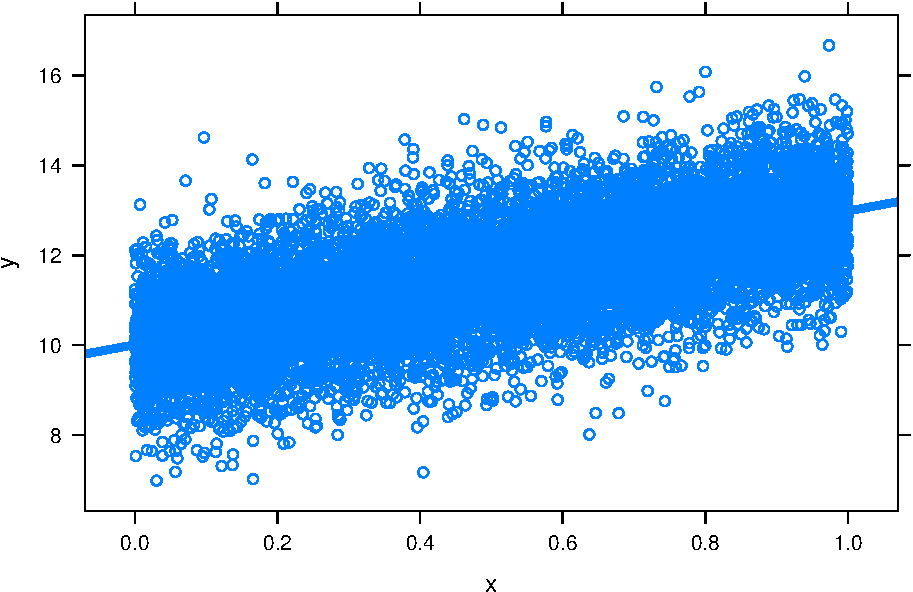
\includegraphics{02_lab_residuals_files/figure-latex/unnamed-chunk-11-1.pdf}

\begin{Shaded}
\begin{Highlighting}[]
\NormalTok{mod1 =}\StringTok{ }\KeywordTok{lm}\NormalTok{(y ~}\StringTok{ }\NormalTok{x, }\DataTypeTok{data=}\NormalTok{ds)}
\KeywordTok{plot}\NormalTok{(mod1, }\DataTypeTok{which=}\DecValTok{1}\NormalTok{)}
\end{Highlighting}
\end{Shaded}

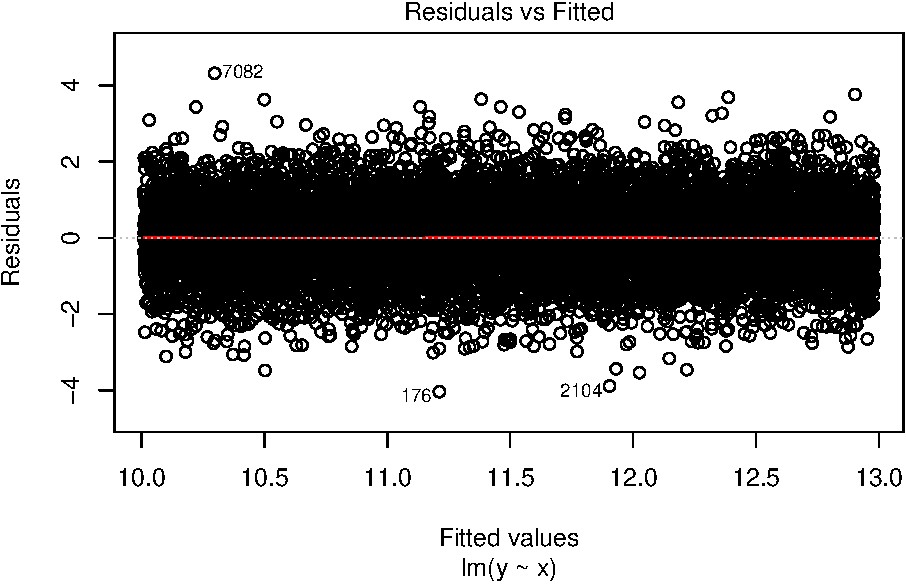
\includegraphics{02_lab_residuals_files/figure-latex/unnamed-chunk-11-2.pdf}

\begin{Shaded}
\begin{Highlighting}[]
\KeywordTok{plot}\NormalTok{(mod1, }\DataTypeTok{which=}\DecValTok{2}\NormalTok{)}
\end{Highlighting}
\end{Shaded}

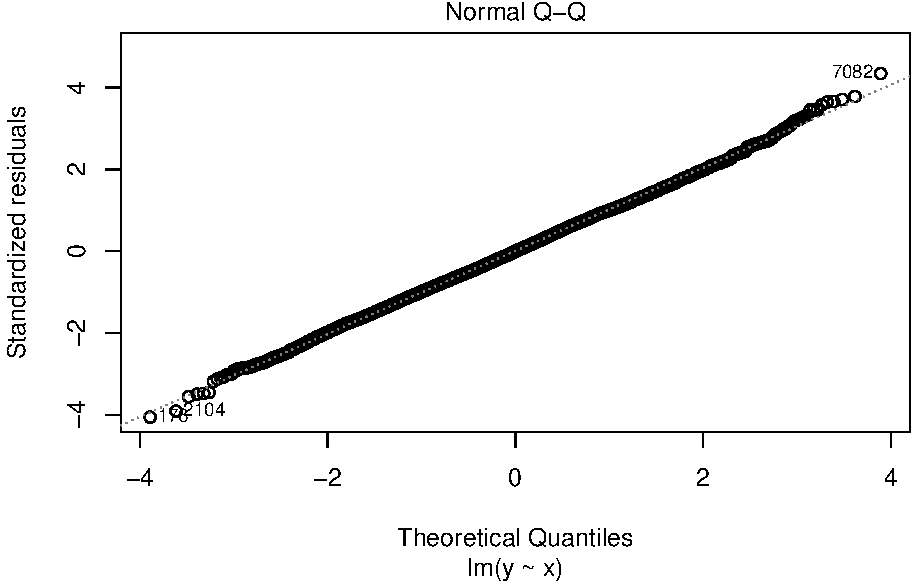
\includegraphics{02_lab_residuals_files/figure-latex/unnamed-chunk-11-3.pdf}

\begin{Shaded}
\begin{Highlighting}[]
\KeywordTok{histogram}\NormalTok{(~}\KeywordTok{residuals}\NormalTok{(mod1), }\DataTypeTok{fit=}\StringTok{"normal"}\NormalTok{)}
\end{Highlighting}
\end{Shaded}

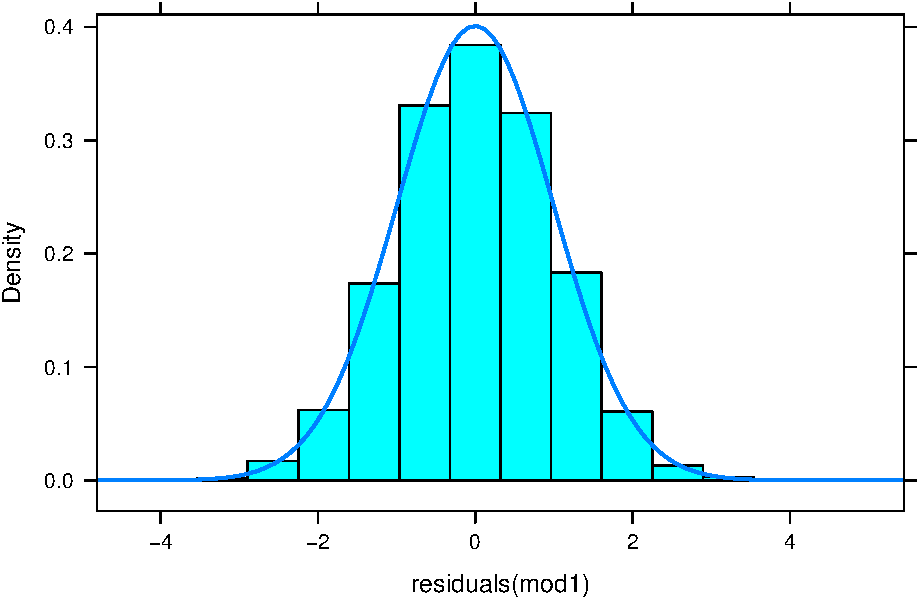
\includegraphics{02_lab_residuals_files/figure-latex/unnamed-chunk-11-4.pdf}

\paragraph{Linearity}\label{linearity}

\begin{Shaded}
\begin{Highlighting}[]
\NormalTok{ds =}\StringTok{ }\KeywordTok{data.frame}\NormalTok{(}\DataTypeTok{y =} \NormalTok{beta0 +}\StringTok{ }\NormalTok{beta1 *}\StringTok{ }\NormalTok{x +}\StringTok{ }\DecValTok{15}\NormalTok{*x^}\DecValTok{2} \NormalTok{+}\StringTok{ }\NormalTok{e)}
\end{Highlighting}
\end{Shaded}

\begin{Shaded}
\begin{Highlighting}[]
\KeywordTok{xyplot}\NormalTok{(y ~}\StringTok{ }\NormalTok{x, }\DataTypeTok{data=}\NormalTok{ds, }\DataTypeTok{type=}\KeywordTok{c}\NormalTok{(}\StringTok{"p"}\NormalTok{, }\StringTok{"r"}\NormalTok{), }\DataTypeTok{lwd=}\DecValTok{5}\NormalTok{)}
\end{Highlighting}
\end{Shaded}

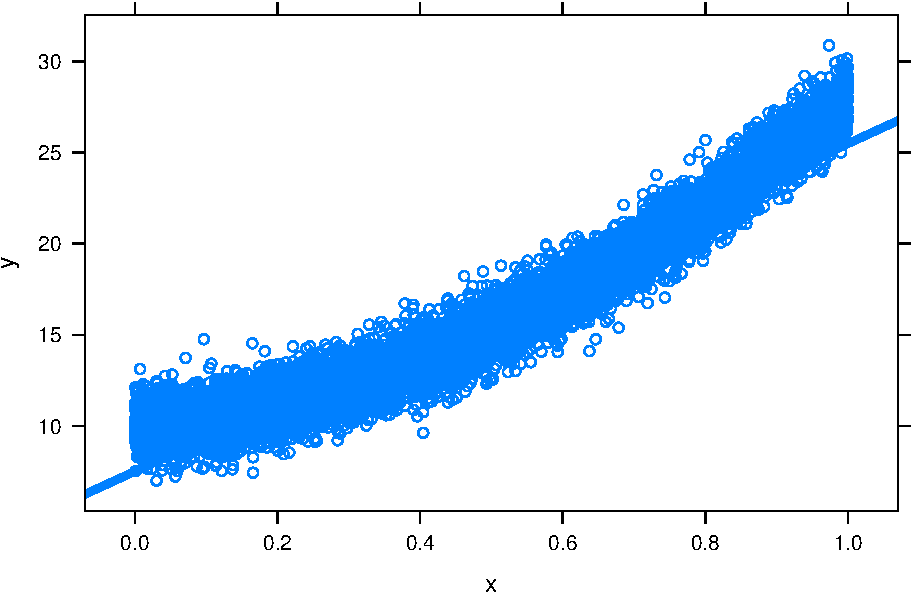
\includegraphics{02_lab_residuals_files/figure-latex/unnamed-chunk-13-1.pdf}

\begin{Shaded}
\begin{Highlighting}[]
\NormalTok{mod2 =}\StringTok{ }\KeywordTok{lm}\NormalTok{(y ~}\StringTok{ }\NormalTok{x, }\DataTypeTok{data=}\NormalTok{ds)}
\KeywordTok{plot}\NormalTok{(mod2, }\DataTypeTok{which=}\DecValTok{1}\NormalTok{)}
\end{Highlighting}
\end{Shaded}

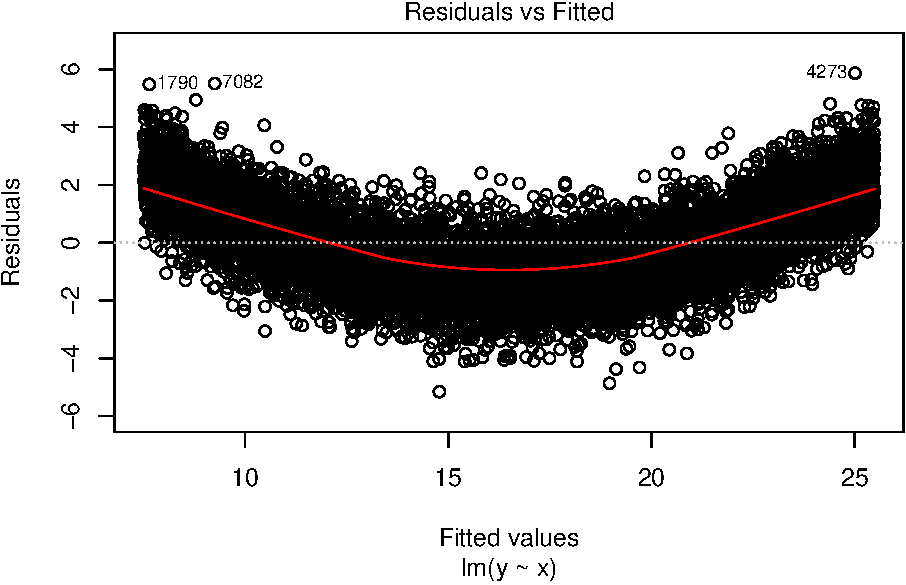
\includegraphics{02_lab_residuals_files/figure-latex/unnamed-chunk-13-2.pdf}

\begin{Shaded}
\begin{Highlighting}[]
\KeywordTok{plot}\NormalTok{(mod2, }\DataTypeTok{which=}\DecValTok{2}\NormalTok{)}
\end{Highlighting}
\end{Shaded}

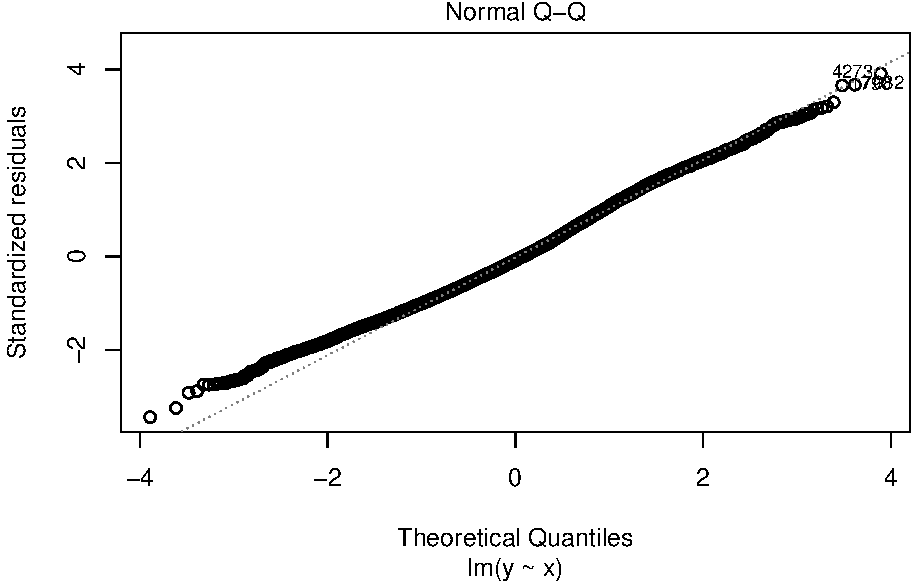
\includegraphics{02_lab_residuals_files/figure-latex/unnamed-chunk-13-3.pdf}

\begin{Shaded}
\begin{Highlighting}[]
\KeywordTok{histogram}\NormalTok{(~}\KeywordTok{residuals}\NormalTok{(mod2), }\DataTypeTok{fit=}\StringTok{"normal"}\NormalTok{)}
\end{Highlighting}
\end{Shaded}

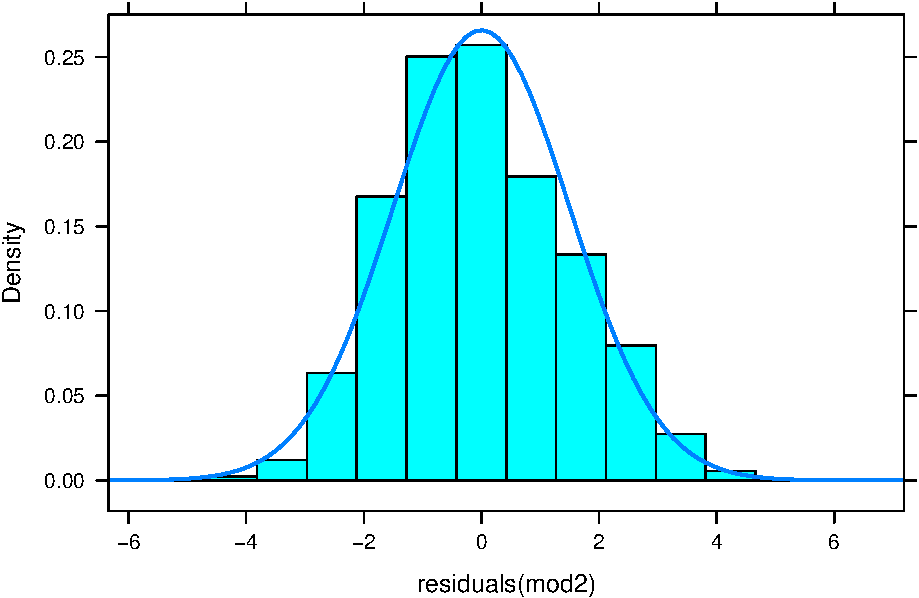
\includegraphics{02_lab_residuals_files/figure-latex/unnamed-chunk-13-4.pdf}

\paragraph{Constant Variance}\label{constant-variance}

\begin{Shaded}
\begin{Highlighting}[]
\NormalTok{ds =}\StringTok{ }\KeywordTok{data.frame}\NormalTok{(}\DataTypeTok{y =} \NormalTok{beta0 +}\StringTok{ }\NormalTok{beta1 *}\StringTok{ }\NormalTok{x +}\StringTok{ }\NormalTok{e*x)}
\end{Highlighting}
\end{Shaded}

\begin{Shaded}
\begin{Highlighting}[]
\KeywordTok{xyplot}\NormalTok{(y ~}\StringTok{ }\NormalTok{x, }\DataTypeTok{data=}\NormalTok{ds, }\DataTypeTok{type=}\KeywordTok{c}\NormalTok{(}\StringTok{"p"}\NormalTok{, }\StringTok{"r"}\NormalTok{), }\DataTypeTok{lwd=}\DecValTok{5}\NormalTok{)}
\end{Highlighting}
\end{Shaded}

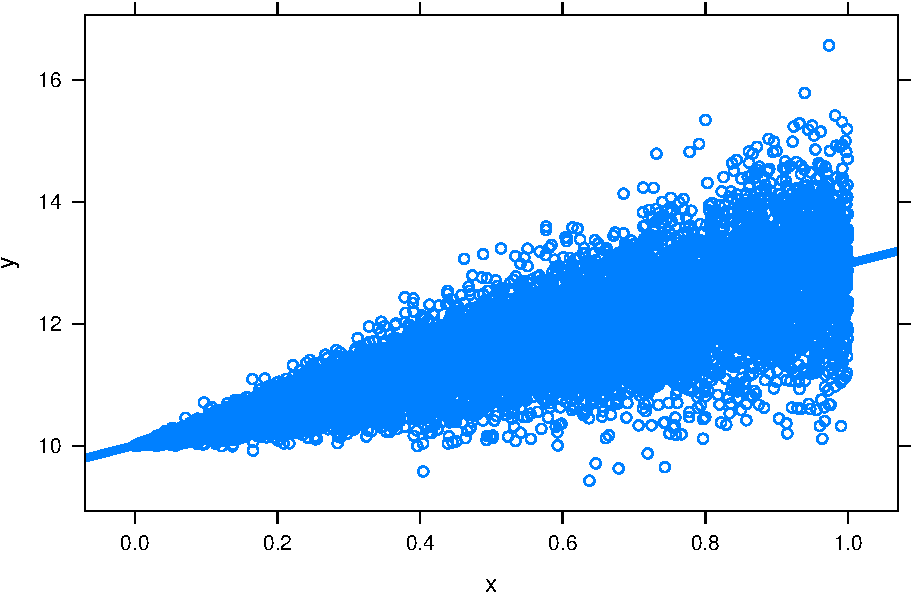
\includegraphics{02_lab_residuals_files/figure-latex/unnamed-chunk-15-1.pdf}

\begin{Shaded}
\begin{Highlighting}[]
\NormalTok{mod3 =}\StringTok{ }\KeywordTok{lm}\NormalTok{(y ~}\StringTok{ }\NormalTok{x, }\DataTypeTok{data=}\NormalTok{ds)}
\KeywordTok{plot}\NormalTok{(mod3, }\DataTypeTok{which=}\DecValTok{1}\NormalTok{)}
\end{Highlighting}
\end{Shaded}

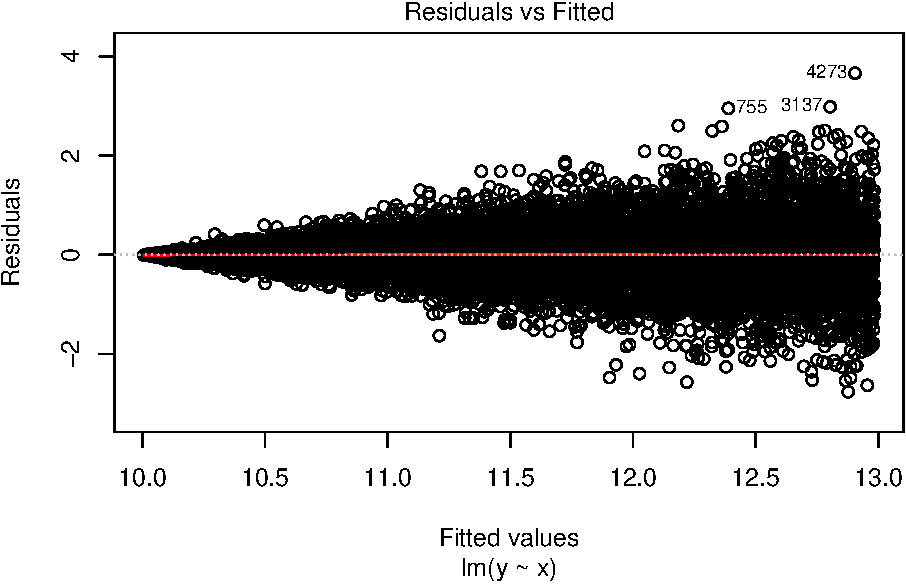
\includegraphics{02_lab_residuals_files/figure-latex/unnamed-chunk-15-2.pdf}

\begin{Shaded}
\begin{Highlighting}[]
\KeywordTok{plot}\NormalTok{(mod3, }\DataTypeTok{which=}\DecValTok{2}\NormalTok{)}
\end{Highlighting}
\end{Shaded}

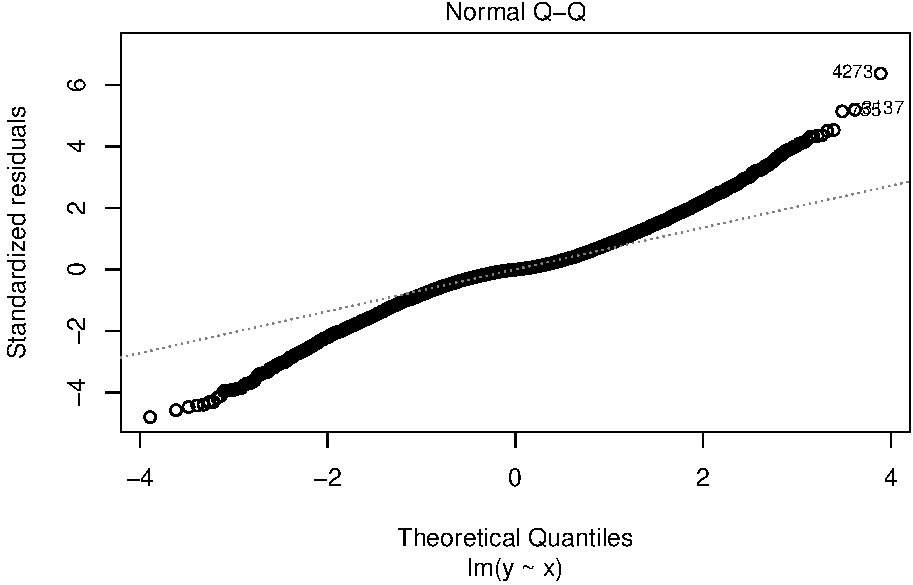
\includegraphics{02_lab_residuals_files/figure-latex/unnamed-chunk-15-3.pdf}

\begin{Shaded}
\begin{Highlighting}[]
\KeywordTok{histogram}\NormalTok{(~}\KeywordTok{residuals}\NormalTok{(mod3), }\DataTypeTok{fit=}\StringTok{"normal"}\NormalTok{)}
\end{Highlighting}
\end{Shaded}

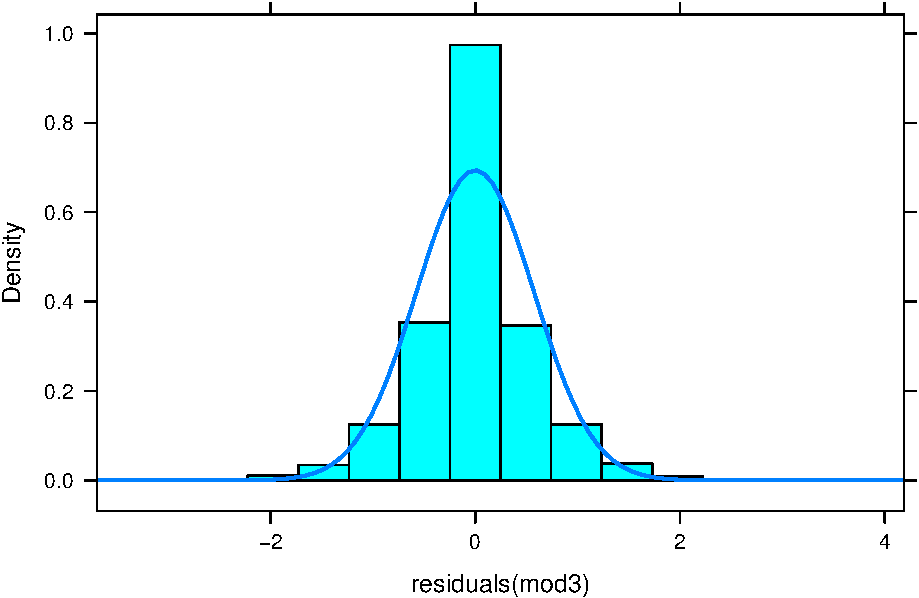
\includegraphics{02_lab_residuals_files/figure-latex/unnamed-chunk-15-4.pdf}

\paragraph{Normality}\label{normality}

\begin{Shaded}
\begin{Highlighting}[]
\NormalTok{ds =}\StringTok{ }\KeywordTok{data.frame}\NormalTok{(}\DataTypeTok{y =} \NormalTok{beta0 +}\StringTok{ }\NormalTok{beta1 *}\StringTok{ }\NormalTok{x +}\StringTok{ }\KeywordTok{rbeta}\NormalTok{(n, }\DataTypeTok{shape1 =} \DecValTok{2}\NormalTok{, }\DataTypeTok{shape2 =} \DecValTok{5}\NormalTok{))}
\end{Highlighting}
\end{Shaded}

\begin{Shaded}
\begin{Highlighting}[]
\KeywordTok{xyplot}\NormalTok{(y ~}\StringTok{ }\NormalTok{x, }\DataTypeTok{data=}\NormalTok{ds, }\DataTypeTok{type=}\KeywordTok{c}\NormalTok{(}\StringTok{"p"}\NormalTok{, }\StringTok{"r"}\NormalTok{), }\DataTypeTok{lwd=}\DecValTok{5}\NormalTok{)}
\end{Highlighting}
\end{Shaded}

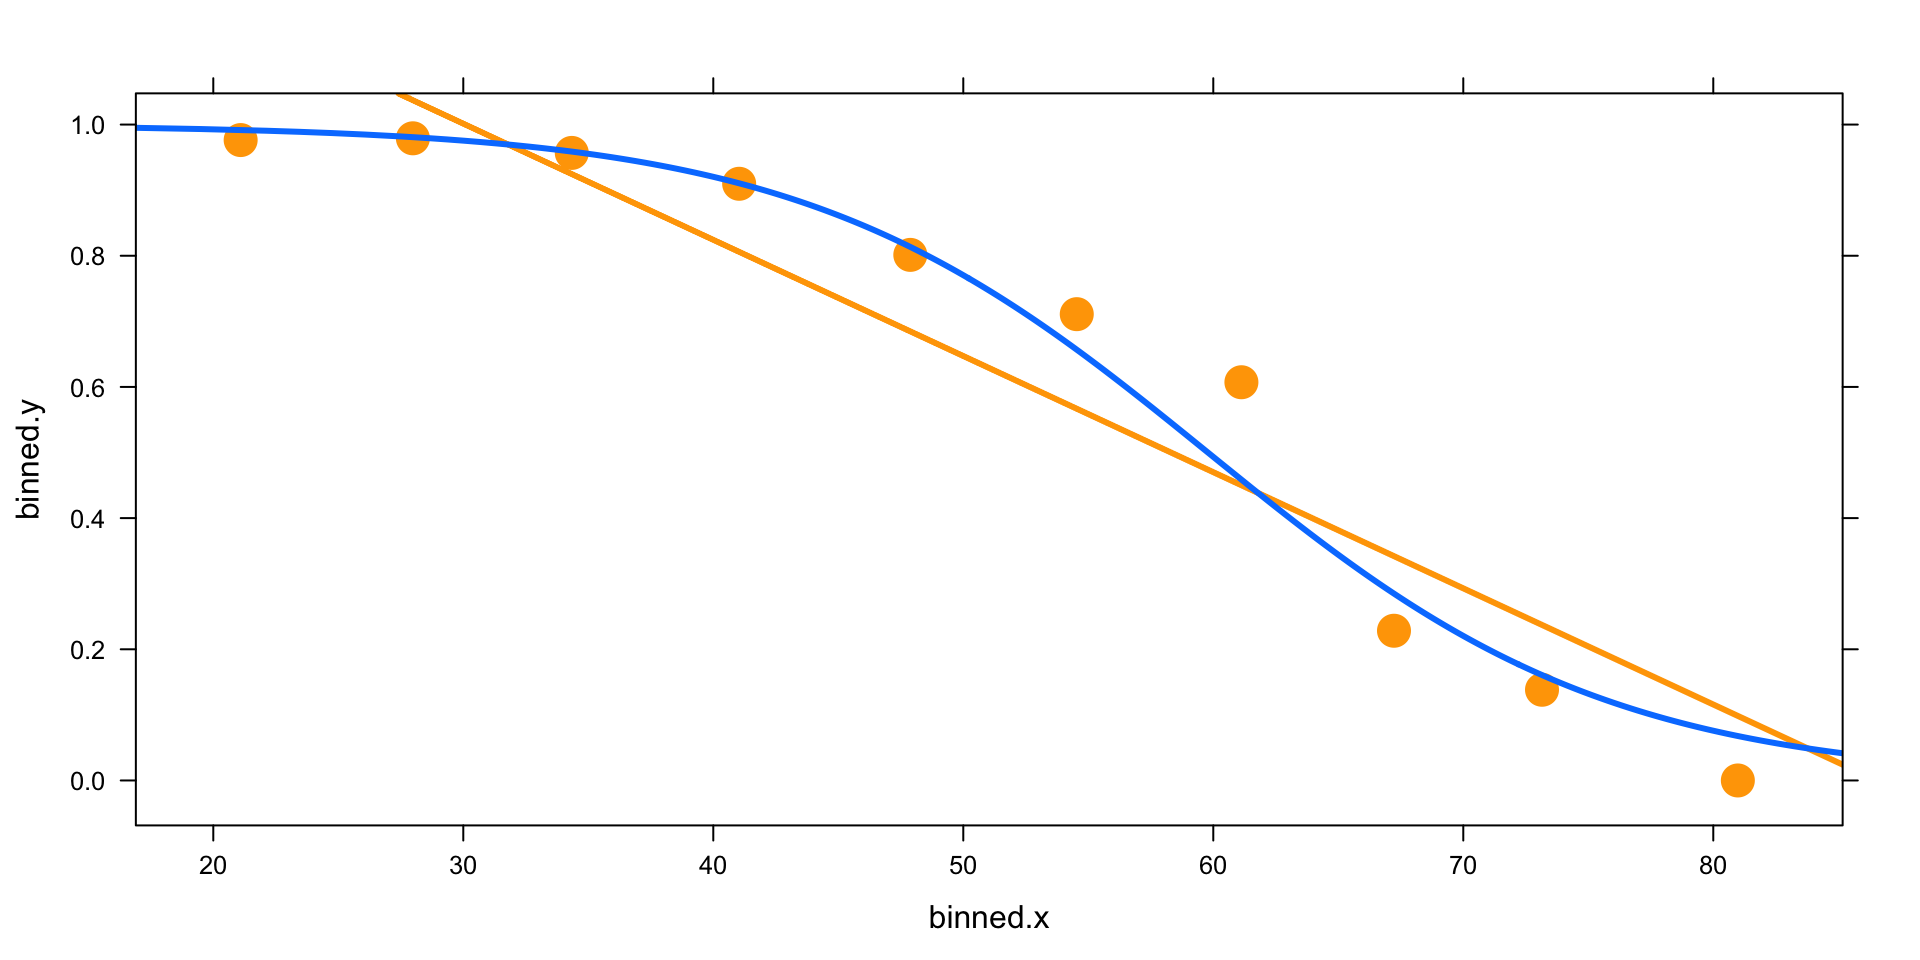
\includegraphics{02_lab_residuals_files/figure-latex/unnamed-chunk-17-1.pdf}

\begin{Shaded}
\begin{Highlighting}[]
\NormalTok{mod4 =}\StringTok{ }\KeywordTok{lm}\NormalTok{(y ~}\StringTok{ }\NormalTok{x, }\DataTypeTok{data=}\NormalTok{ds)}
\KeywordTok{plot}\NormalTok{(mod4, }\DataTypeTok{which=}\DecValTok{1}\NormalTok{)}
\end{Highlighting}
\end{Shaded}

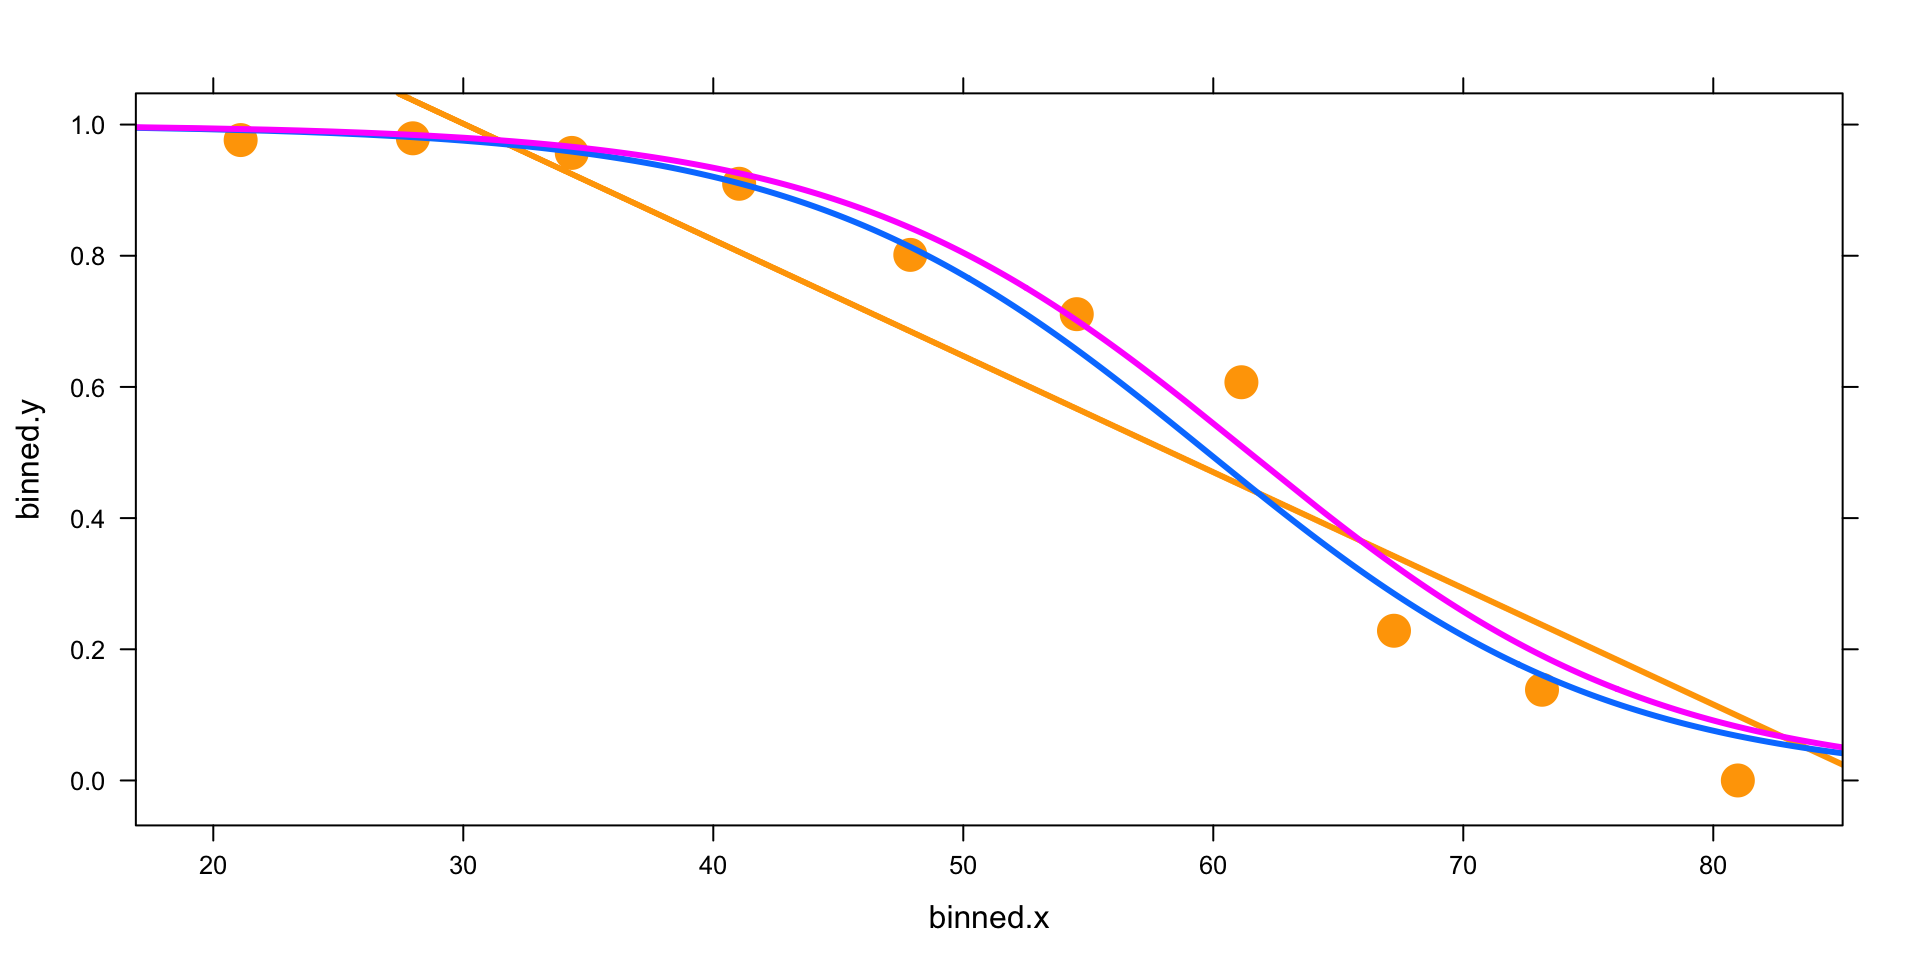
\includegraphics{02_lab_residuals_files/figure-latex/unnamed-chunk-17-2.pdf}

\begin{Shaded}
\begin{Highlighting}[]
\KeywordTok{plot}\NormalTok{(mod4, }\DataTypeTok{which=}\DecValTok{2}\NormalTok{)}
\end{Highlighting}
\end{Shaded}

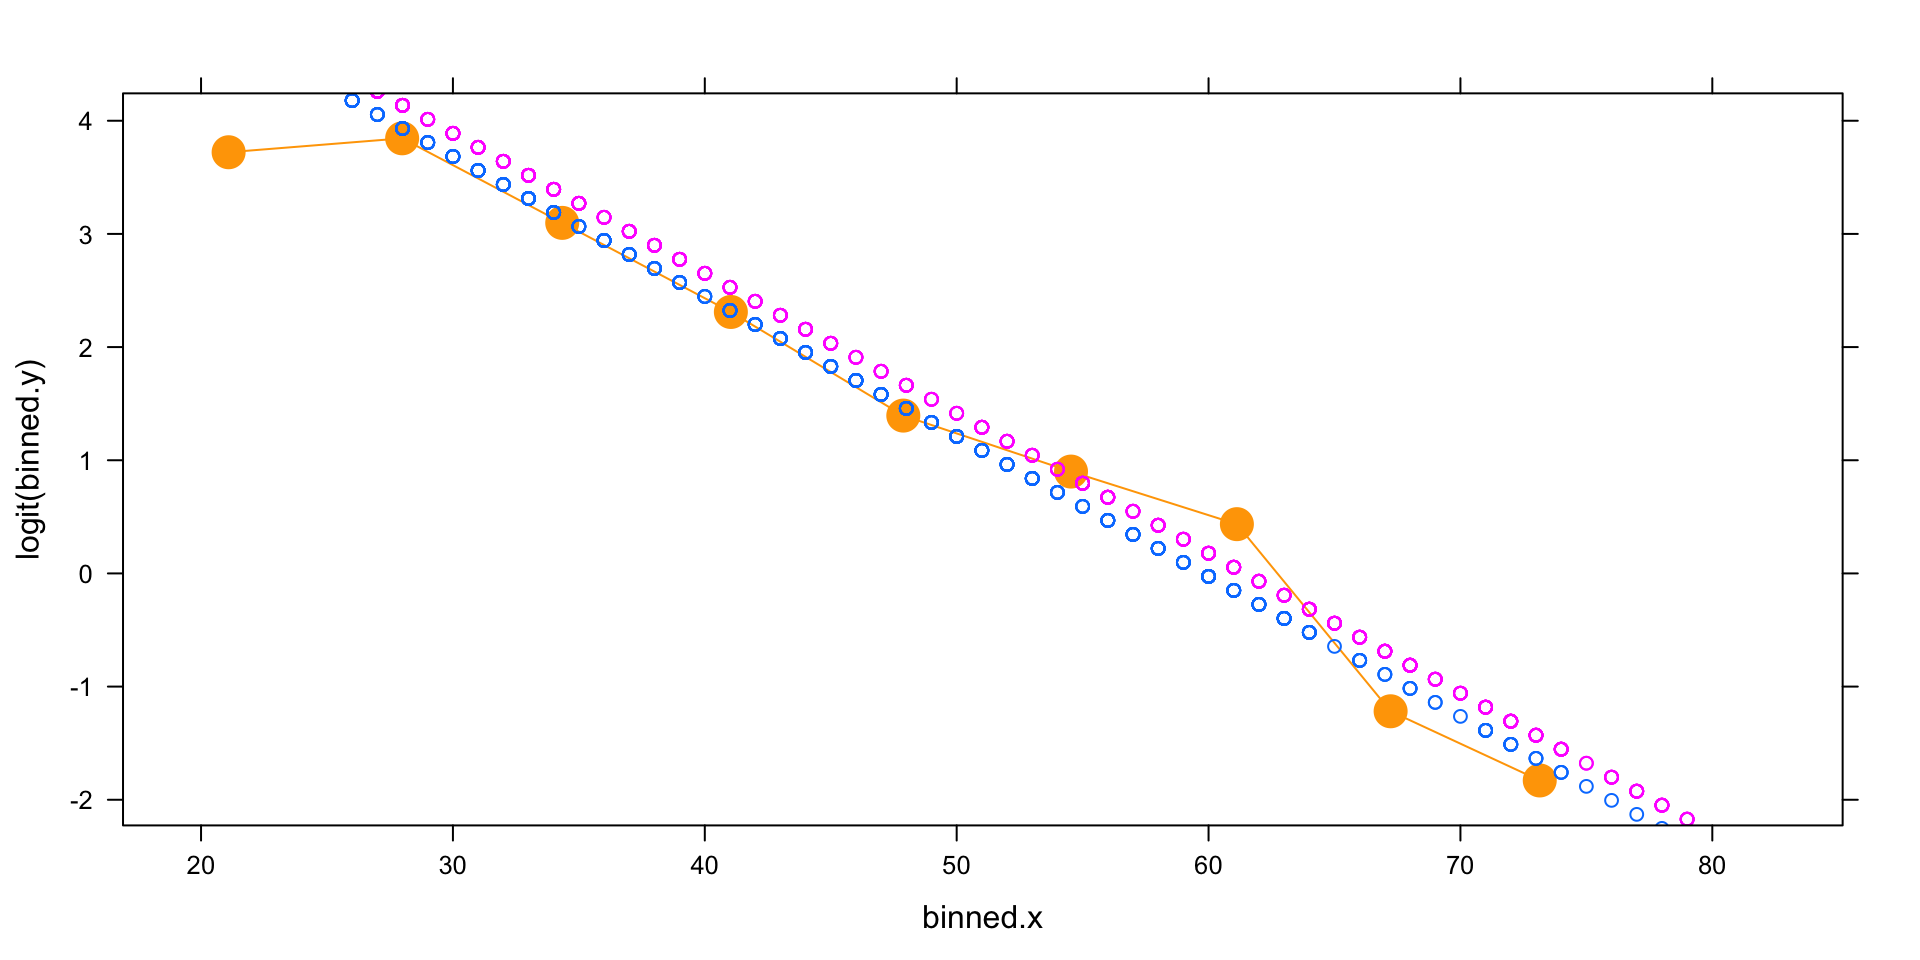
\includegraphics{02_lab_residuals_files/figure-latex/unnamed-chunk-17-3.pdf}

\begin{Shaded}
\begin{Highlighting}[]
\KeywordTok{histogram}\NormalTok{(~}\KeywordTok{residuals}\NormalTok{(mod4), }\DataTypeTok{fit=}\StringTok{"normal"}\NormalTok{)}
\end{Highlighting}
\end{Shaded}

\includegraphics{02_lab_residuals_files/figure-latex/unnamed-chunk-17-4.pdf}

\paragraph{How much is too much?}\label{how-much-is-too-much}

How loosely should we allow the conditions for regression to be
violated? To get a feel for this, consider the following simulation.
Note that, by construction, the data are generated from the model: \[
  Y = 10 + 3 \cdot X + \epsilon, \qquad \epsilon \sim N(0, 1)
\]

\begin{Shaded}
\begin{Highlighting}[]
\KeywordTok{require}\NormalTok{(mosaic)}
\NormalTok{n =}\StringTok{ }\DecValTok{20}
\NormalTok{ds =}\StringTok{ }\KeywordTok{data.frame}\NormalTok{(}\DataTypeTok{x =} \KeywordTok{rnorm}\NormalTok{(n))}
\NormalTok{ds =}\StringTok{ }\NormalTok{ds %>%}
\StringTok{  }\KeywordTok{mutate}\NormalTok{(}\DataTypeTok{y =} \DecValTok{10} \NormalTok{+}\StringTok{ }\DecValTok{3} \NormalTok{*}\StringTok{ }\NormalTok{x +}\StringTok{ }\KeywordTok{rnorm}\NormalTok{(n))}
\KeywordTok{xyplot}\NormalTok{(y ~}\StringTok{ }\NormalTok{x, }\DataTypeTok{data=}\NormalTok{ds, }\DataTypeTok{type=}\KeywordTok{c}\NormalTok{(}\StringTok{"p"}\NormalTok{, }\StringTok{"r"}\NormalTok{))}
\end{Highlighting}
\end{Shaded}

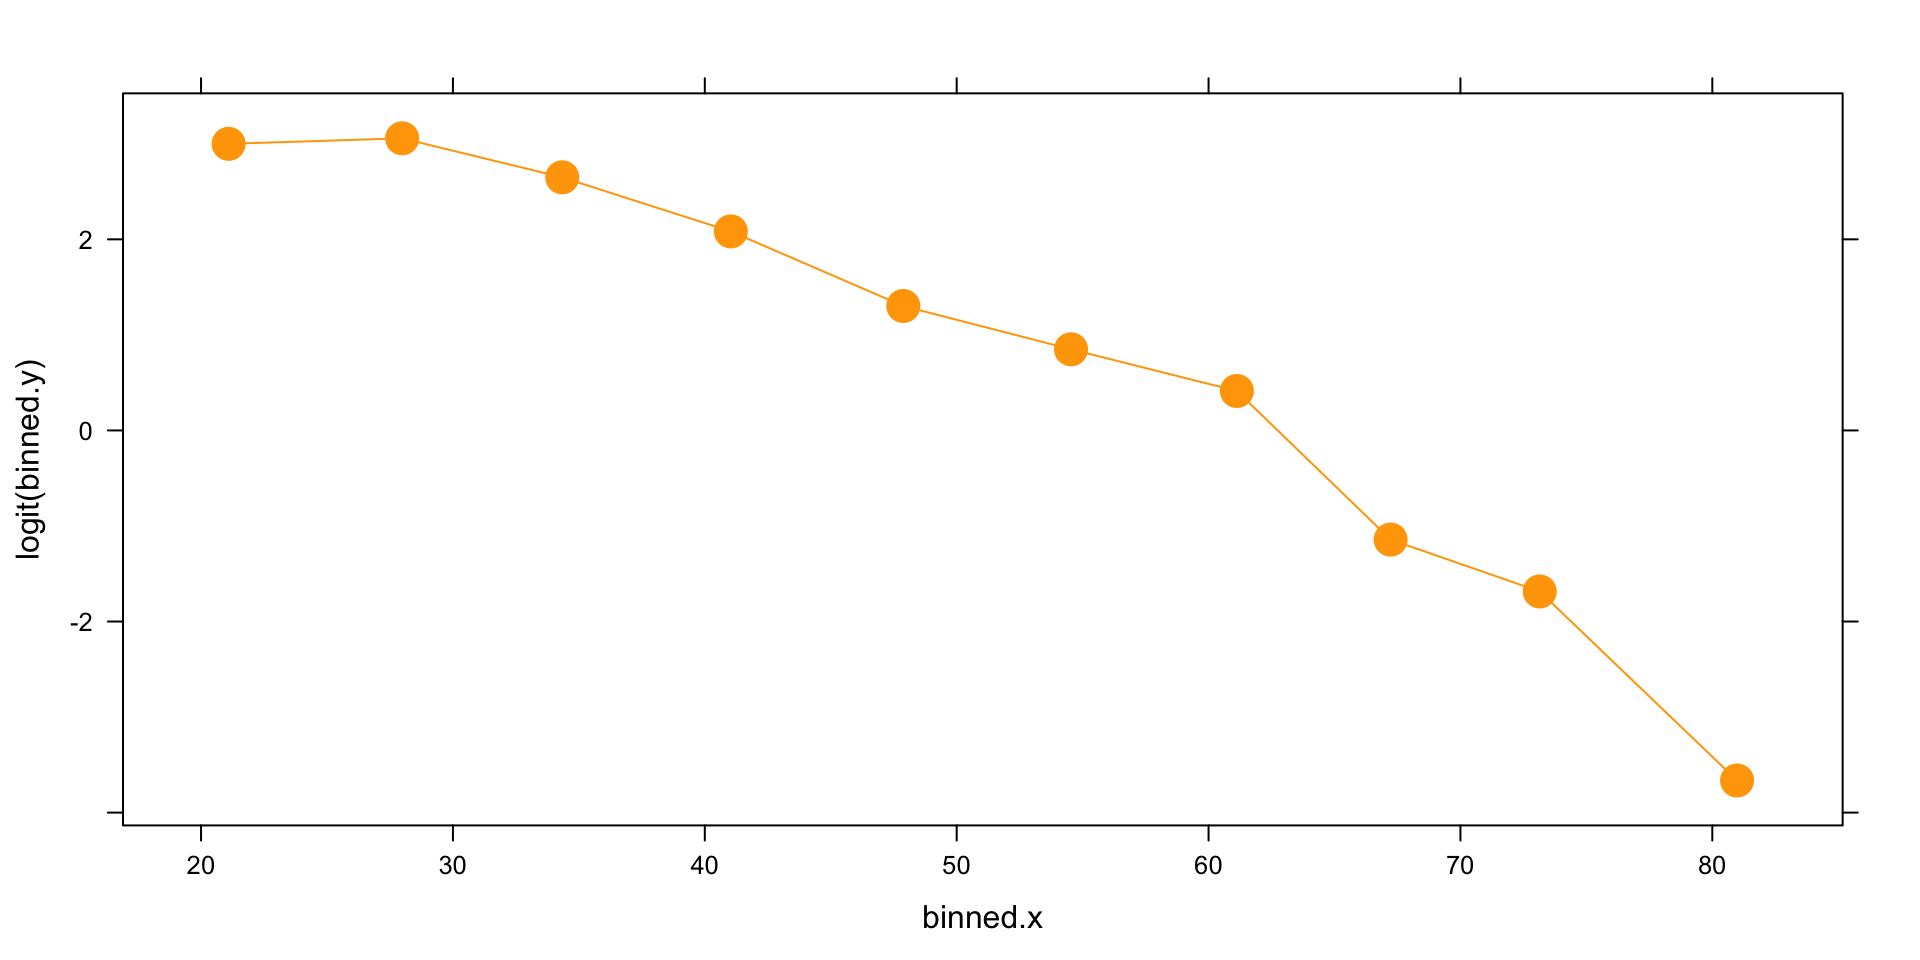
\includegraphics{02_lab_residuals_files/figure-latex/unnamed-chunk-18-1.pdf}

\begin{Shaded}
\begin{Highlighting}[]
\NormalTok{mod_ex <-}\StringTok{ }\KeywordTok{lm}\NormalTok{(y ~x, }\DataTypeTok{data=}\NormalTok{ds)}
\KeywordTok{plot}\NormalTok{(mod_ex, }\DataTypeTok{which=}\KeywordTok{c}\NormalTok{(}\DecValTok{1}\NormalTok{,}\DecValTok{2}\NormalTok{))}
\end{Highlighting}
\end{Shaded}

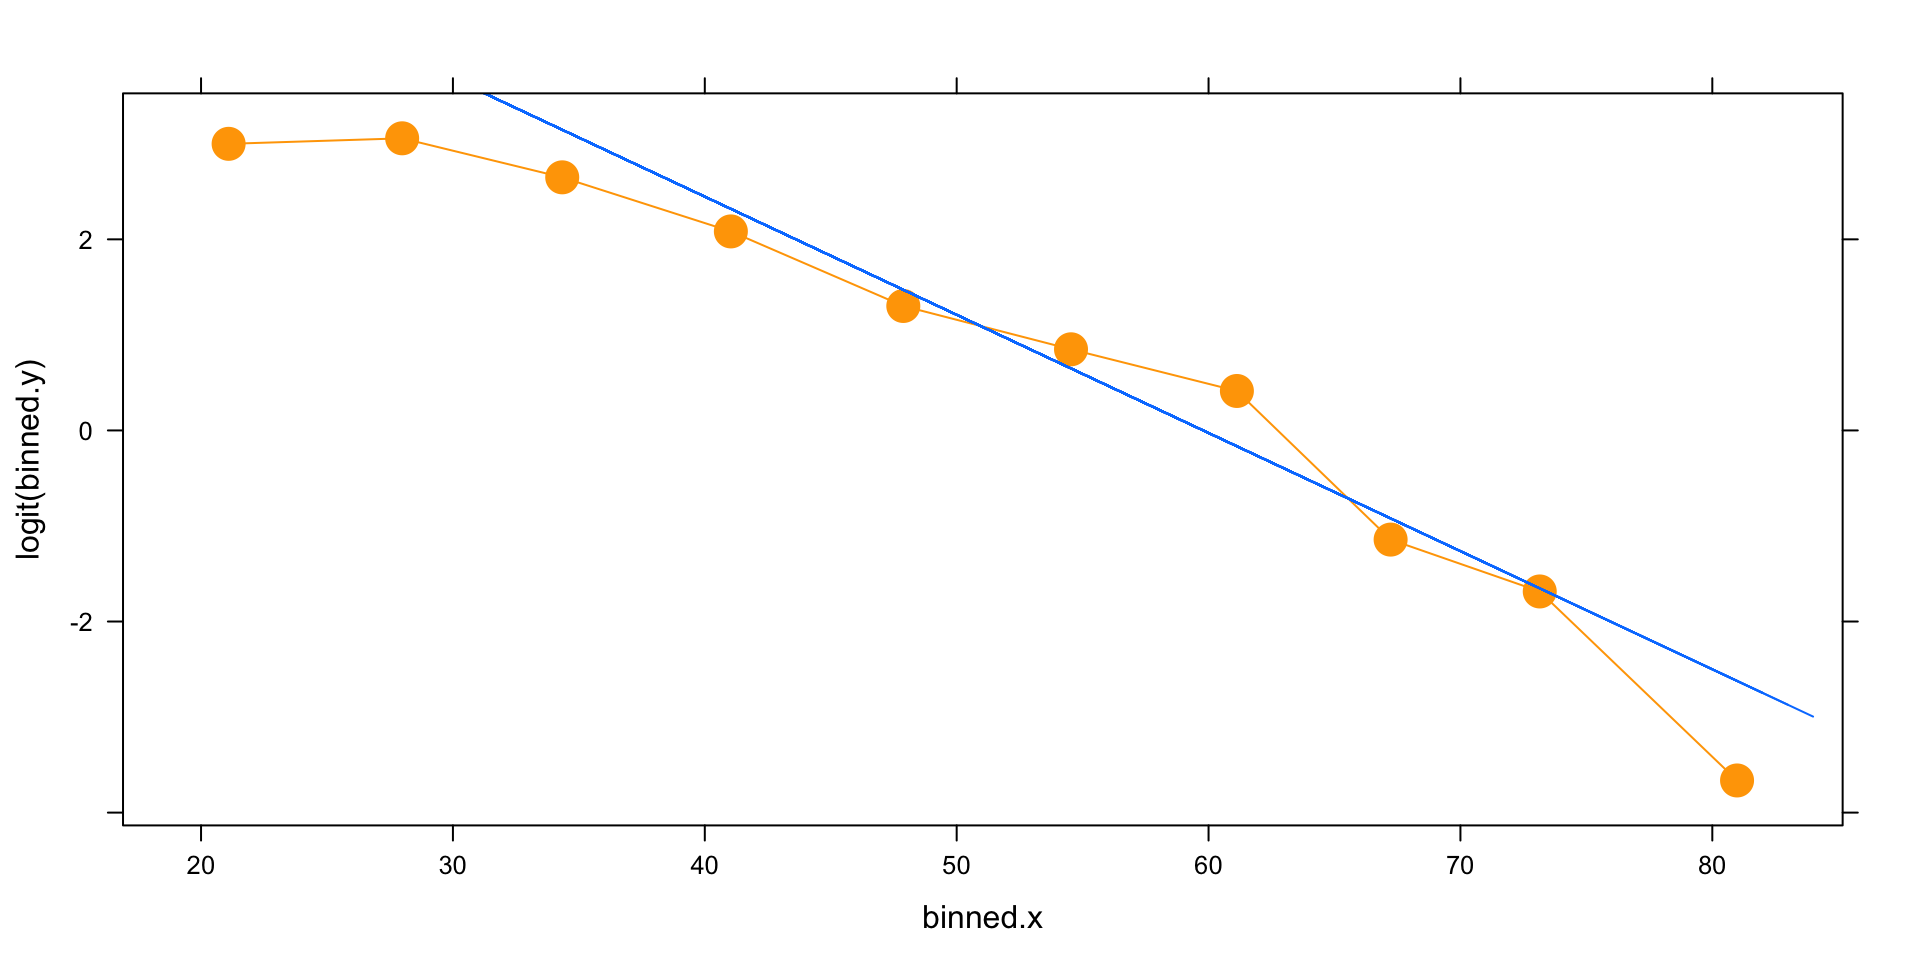
\includegraphics{02_lab_residuals_files/figure-latex/unnamed-chunk-18-2.pdf}
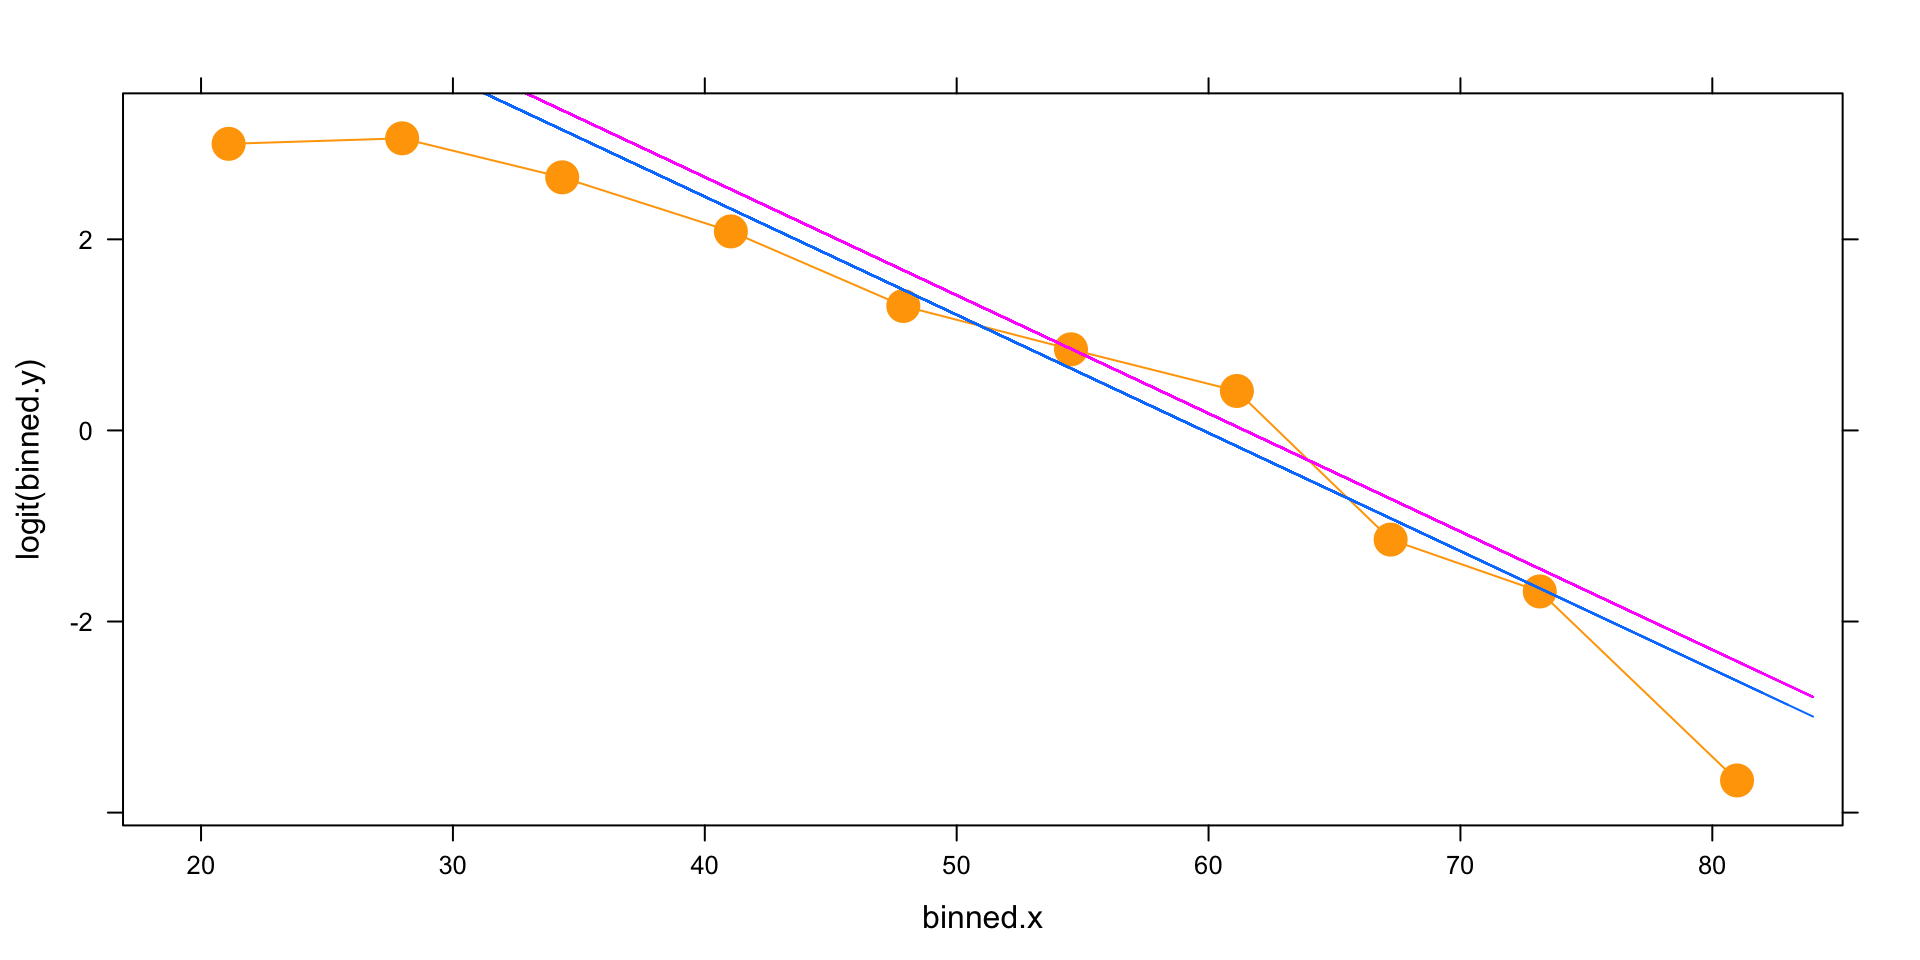
\includegraphics{02_lab_residuals_files/figure-latex/unnamed-chunk-18-3.pdf}

Run this chunk several times, with several different choices of \(n\).
What do you notice?

\end{document}
